\documentclass{article}
\usepackage[utf8]{inputenc}
\usepackage{graphicx}
\usepackage{biblatex}
\usepackage{blindtext}
\usepackage[section]{placeins}
\usepackage{amsmath}
\addbibresource{citing.bib}
\graphicspath{ {./image/} }
\title{Git Assignment}
\author{Moses Smith Guddah}
\date{September 21 2021}

\subsection*{Section I:  Introduction }

I am a Ph.D. student and Graduate Teaching Assistant with the College of Engineering and Applied Science, University of Colorado, Colorado Springs (UCCS). My research interests focus on High Performance Computing systems with specific focus on memory management for Load balancing systems. 

Even though I have had some research experience in Business Management, this course syllabus presents aspects of Computer Science research broadly and very differently from what I have previously done in Business. It is my hope this course enables me understand the knowledge required for being an excellent Computer Science researcher. Further, it is my desire to use the knowledge gained through this course for publishing papers, which is a cardinal part of my Ph.D. program.  

I have worked in the telecommunication industry over the last fifteen years as a Network Deployment Engineer, Intelligent Network Engineer, Network Administrator and a Project Administrator. Those fifteen years allowed my teams deploy cutting-edge technologies in developing country across some regions of Africa that improved mobile communication.

On a personal level, my broader interests lie in understanding how cultural dynamics and micro politics within scientific communities, and public policies impact quality scientific research. There is a schism between science, and politics and culture that has confronted society. Though much has been done to narrow that divide, there is definitely more of understand and influence, so that policy- makers can support scientific communities for significant and impacting research. I am an ardent Tennis player and a  lover of running  trails.

I am married to an intelligent, beautiful, resourceful lady, Jemu Zarzar- Guddah and we have a two-year-old daughter.

\begin{figure}[hbt!]
    \centering
    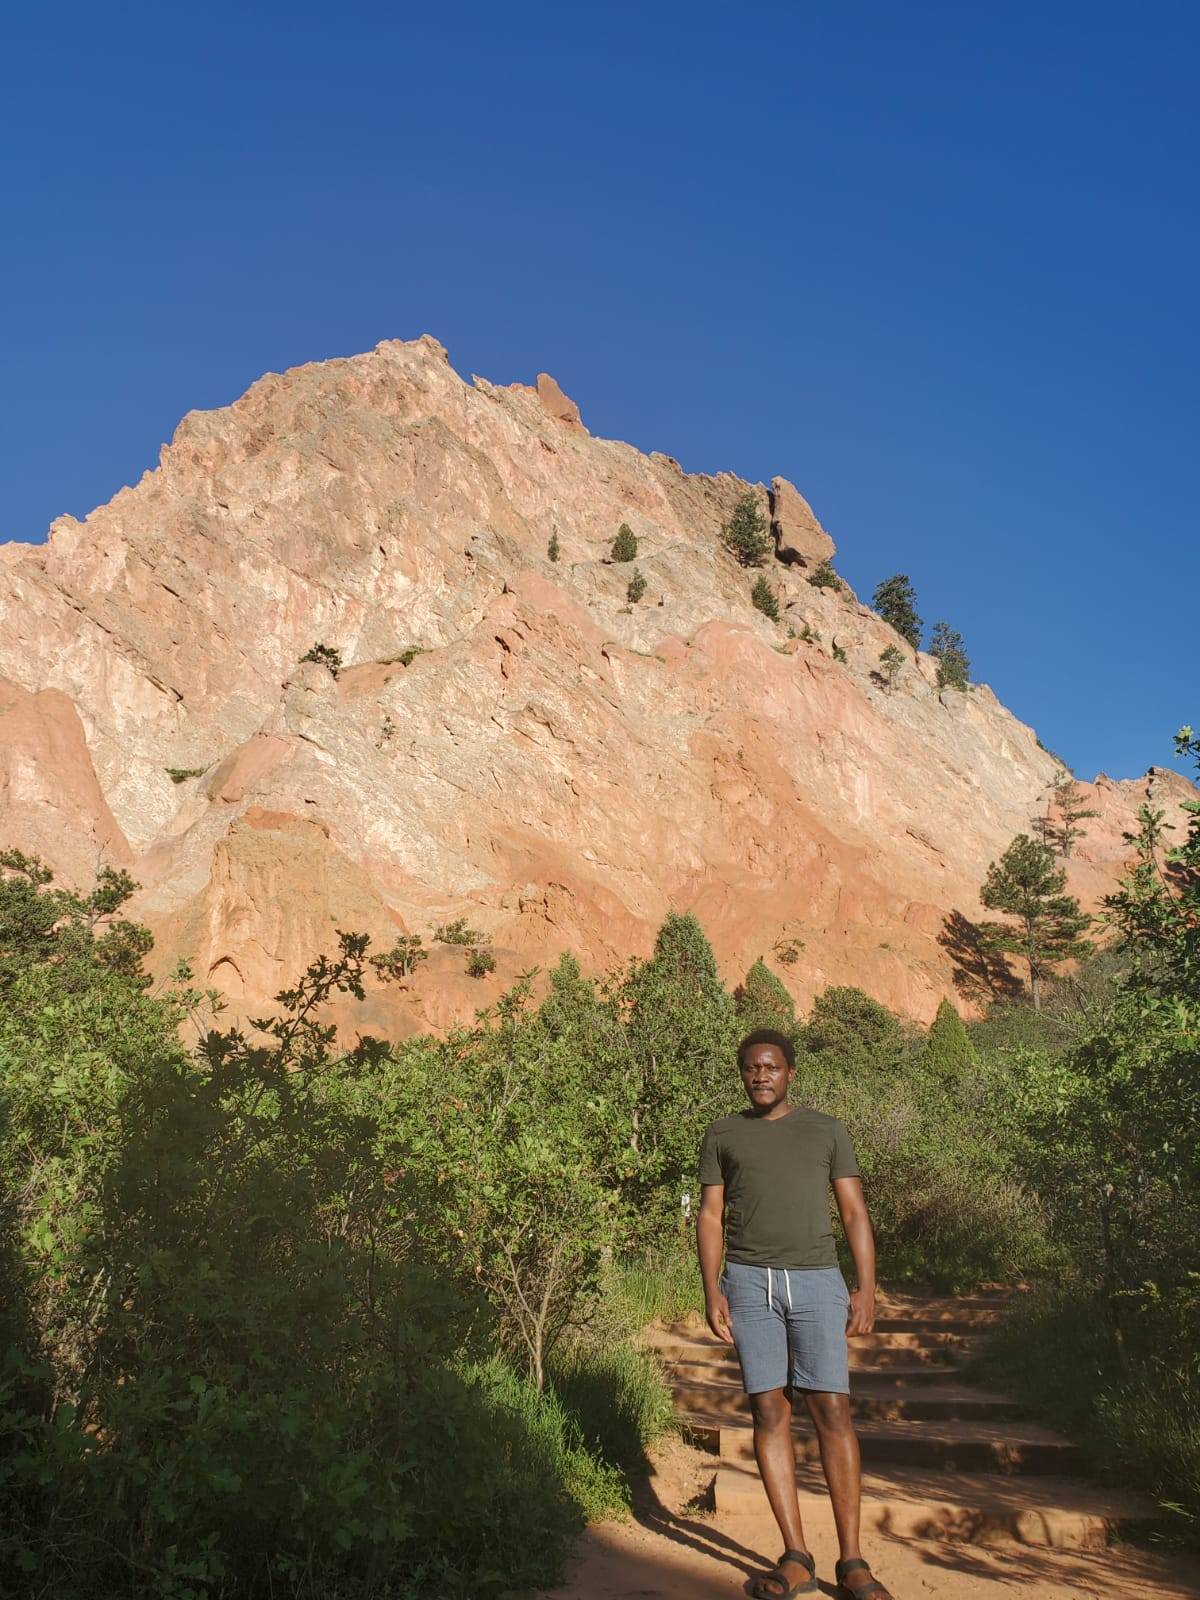
\includegraphics[width=7cm, height=8cm]{TrailWalk}
    \caption{A trail walk in Garden of the Gods, Colorado Springs}
\end{figure}


\subsection*{Section II:  Research Area}
Latency and throughput remain critical performance requirements for internet-based applications in distributed environments such as the cloud-based architecture. Though there have been significant research  done on load balancing in cloud computing environments, a bulk of the research have focused primarily on implementing elasticity in the computing environment by scaling-up(vertical scalability) or  scaling-out(horizontal scalability) \cite{raghava2014comparative,velde2017advanced}. However, a crucial aspect of performance in any cloud architecture is cost of performance as the infrastructure is scaled. MBal\cite{cheng2015memory,hong2013understanding,chavan2014clustered} provides a fundamental approach on orchestrating in-memory technique that presents benefits of cost reduction to cloud users.

MBal proposes two objective functions based on Integer Linear Programming(ILP). The goal of the first function, presented below,  minimizes count of migration operations with a fixed source worker.\\

minimize  
\begin{eqnarray}
    \sum_{i}\sum_{j}X_{ij}^{k} \\
s.t. \    L_{*a} +  \sum_{i}\sum_{j}X_{ia}^{k}L_{i}^{k} -   \sum_{i}\sum_{j}X_{ia}^{k}L_{a}^{k} \leq T_{a}\\
\forall i \in S \backslash a: L_{*i}+\sum_{k}X_{ia}^{k}L_{i}^{k} - \sum_{k}X_{ia}^{k}L_{i}^{k}\leq T_{i}
\end{eqnarray}


where a is the index of the fixed source worker thread; $X_{ij}^{k}$ is 1 if the cachetlet k is migrated from worker i to worker j, 0 otherwise; $ T_{j} $ is the maximum permissible load on worker j; $ L_{*j} $ is the total load on worker j. 

The below git repos has relevance to my research even though it is rudimentary. It provides a read/write memory function based on process id. It can be found at \url{https://github.com/voyula/read-write-memory/blob/master/src/read-write-memory.cpp}


\clearpage
\nocite{*}
\printbibliography
